\section{Batch processing with Stratosphere}\label{stratosphere}

\begin{figure*}
\centering
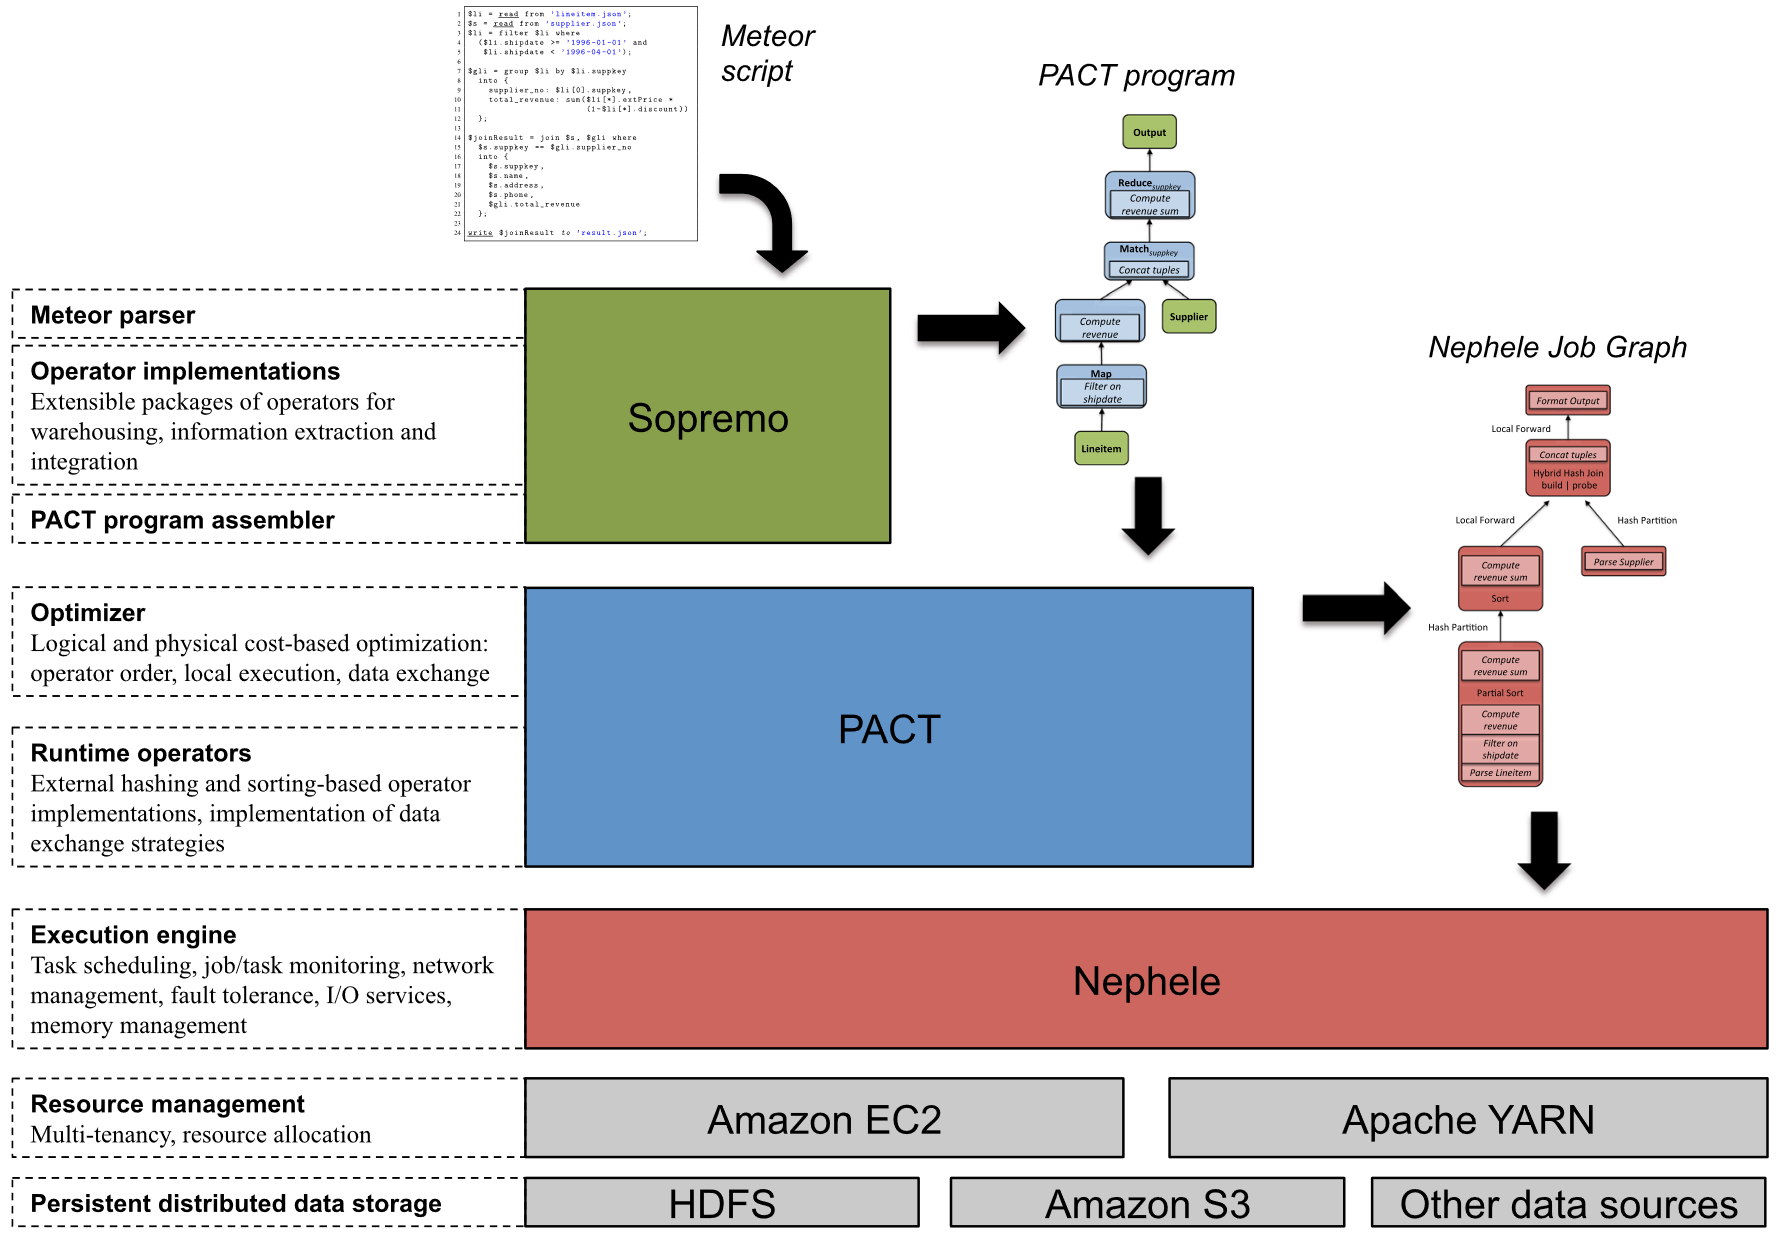
\includegraphics[width=7.0in]{./img/StratosphereSystemOverview.png}
\caption{Stratosphere system overview. Notice the layered system that connects to several different popular file systems~\cite{Stratosphere2014}.}
\label{fig_stratosphere_overview}
\end{figure*}

The Stratosphere project was a research project by institutes of Technical University Berlin, Humboldt University Berlin and Hasso Plattner Institute Potsdam. It was founded in 2009 and continued with publications until 2016~\cite{StratospherePublications}. After research on parts of the system had advanced far enough, the combined system was introduced as ``The Stratosphere platform for big data analytics" in 2014~\cite{Stratosphere2014}. The goal of the project was ``to jointly research and build a large-scale data processor based on concepts of robust and adaptive execution"~\cite{StratosphereDIMA} and for the user to be able to comfortably execute analytical tasks on large batches of data~\cite{Stratosphere2014}. Also in 2014, the project evolved into a Apache top level project under the name of Apache Flink~\cite{StratospherePublications}. As for Aurora, we will now – referring to~\cite{Stratosphere2014} - describe the reasons for developing a system like Stratosphere and afterwards explain its main components.

\subsection{Problems of batch processing with traditional RDBMSs}\label{batchRDBMSProblems}
Similar to stream processing, traditional (parallel) RDBMSs are able to perform analytical tasks on large batches of data, but again they are slow and inefficient at this task. In addition, RDBMSs have difficulties in handling semi-structured and unstructured data, which is a issue, because many analytical tasks are performed on such data. Finally, the authors add, there is little comfort from the user's point of view in using RDBMSs, thus making the work inefficient.

\subsection{Stratosphere system overview}\label{stratosphereOverview}
To address the issues of processing large amounts of data at once and in a reasonable time, Stratosphere offers several features. First, it performs in-situ data processing, thereby minimizing memory usage. Second, Stratosphere offers a declarative query language. The authors think that the high level of abstraction, which declarative languages offer, makes users more productive. Furthermore, the system automizes program parallelization and optimization and has a scalable, distributed execution engine. User defined functions are treated as first class citizens and the set of operators is extensible. Last, Stratosphere supports iterative programs by default. Because of those features, Stratosphere is useful in many use cases, such as data warehousing, information extraction, data cleansing, graph analysis and statistical analysis.

The system consists of several layers, as seen in Fig.~\ref{fig_stratosphere_overview}. Queries are written in Meteor, Stratosphere's declarative query language. A Meteor script is translated into a directed, acyclic graph (DAG) by the Sopremo layer. PACT then further translates the Sopremo DAG by braking Sopremo operators down to PACT operators, which consist of five pre-implemented second order functions combined with user defined functions (UDFs). Afterwards, the PACT DAG gets optimized in four steps, resulting in a Nephele Job Graph. Nephele is Stratosphere's parallel execution engine and takes care of scheduling tasks on different worker nodes. The system can connect to several popular file systems, including YARN~\footnote{\url{https://hadoop.apache.org/docs/current/hadoop-yarn/hadoop-yarn-site/YARN.html}}, Amazon EC2~\footnote{\url{https://aws.amazon.com/de/ec2/}}, and Hadoop Distributed File System~\footnote{\url{https://hadoop.apache.org/docs/r1.2.1/hdfs_design.html}}. Note that queries can be either input as Meteor scripts, Sopremo graphs or PACT programs. That allows different levels of abstraction regarding queries.

\subsection{Meteor and Sopremo}\label{stratosphereSopremo}

\begin{figure}[!t]
\centering
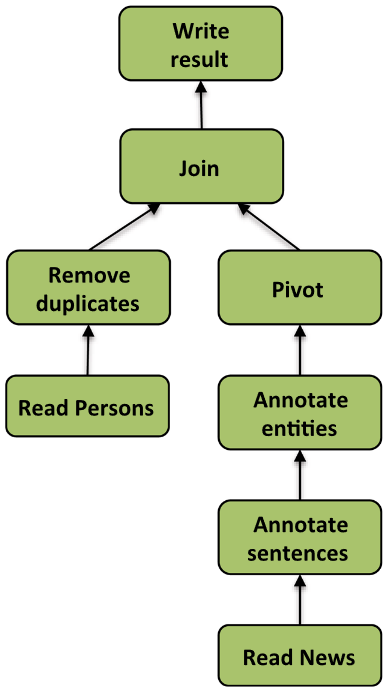
\includegraphics[width=1.5in]{./img/SopremoDAG.png}
\caption{A directed acyclic graph (DAG) in the Sopremo layer. Sopremo can take a DAG as an input or translate a Meteor script to a DAG~\cite{Stratosphere2014}.}
\label{fig_stratosphere_sopremo_dag}
\end{figure}

Meteor serves as the query language for the topmost Sopremo layer. Thereby, Meteor abstracts queries from a Sopremo graph into a structured query language. This relation implies that every Meteor operator must be backed by a corresponding Sopremo operator. An example Sopremo DAG is shown in Fig.~\ref{fig_stratosphere_sopremo_dag}. Each node in the DAG resembles a Meteor operation and each Meteor variable is represented by a vertex in the graph. Sopremo operators may be elemental or composed out of elemental operators. As of 2014, Sopremo already supported a wide range of operations for Meteor. A detailed listing of supported operations is shown in~\cite{Stratosphere2014}.

\subsection{PACT}\label{straotspherePACT}

\begin{figure}[!t]
\centering
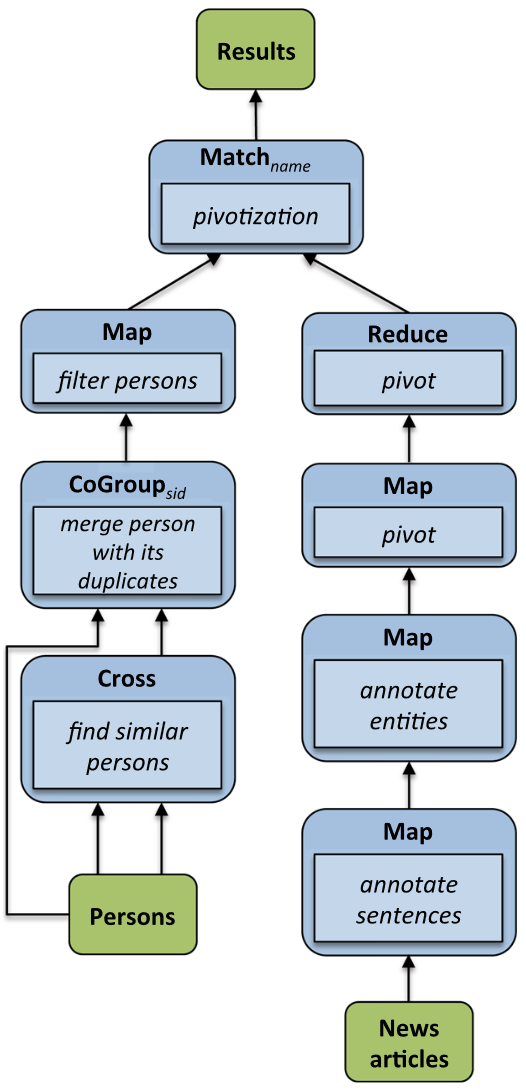
\includegraphics[width=1.5in]{./img/PACTDAG.png}
\caption{DAG of a PACT program. Every Sopremo operator has to be backed by a PACT operator or program~\cite{Stratosphere2014}.}
\label{fig_pact_dag}
\end{figure}

The PACT layer's job is to provide information about parallelization. PACT stands for ``parallelization contract". Each PACT operator, or simply PACT, consists of a second order function and a UDF. Stratosphere started with a set of five PACT second order functions in 2014: \textit{Map, Reduce, Cross, Match, and CoGroup}. The purpose of the second order functions is that each of them forms different \textit{parallelization units} (PU) when processing data. For example, \textit{Reduce} creates a PU for each key of the input. The PUs define the way that incoming data may be distributed to different computers. Because a second order function itself describes only how data is grouped into PUs, each PACT needs a UDF to actually perform any operation on the data. Each Sopremo operator must be backed by a PACT, consisting of a second order function and an implemented UDF. The set of second order functions, as well as the set of pre-implemented PACTs backing Sopremo operators is extensible. That allows power users to freely extend the operator set. For example, a company could decide to implement a PACT for a complex function, that is often used in the company's working context, and must otherwise be composed out of many Sopremo operators.

Because many data analysis tasks can not be algorithmically solved in one iteration, the PACT programming model supports iterative programs. Such programs can either perform \textit{bulk iterations} or \textit{incremental iterations}. A \textit{bulk iteration} consumes the whole data set in each iteration and a \textit{incremental iteration} has a result set and a working set. Only the working set is consumed by the iteration, modifying the result set after each iteration.

Because it supports more operators than MapReduce and natively embeds iterative operations, the PACT model can be seen as a generalization of MapReduce's operator model.

PACT transforms a Sopremo DAG into a PACT DAG by translating each Sopremo operator into the corresponding PACT operator(s). Fig.~\ref{fig_pact_dag} shows the result of the translation of the Sopremo graph from Fig.~\ref{fig_stratosphere_sopremo_dag}.

\subsection{Stratosphere's Optimizer}\label{straotsphereOptimizer}
Before a program gets executed, it is optimized. First, the PACT DAG gets translated to a internal representation. Data sources and sinks, as well as some internal operations are added to the DAG. Afterwards, the optimization itself is performed in two stages. The first stage, logical optimization, consists of the reordering of operators. Because the system does not use relational algebra, traditional rules for reordering, such as the commutative property, do not apply. The UDFs make it difficult to generalize reordering rules. The authors developed two conditions, under which two operators may be switched. First, there may be no conflicting read and write operations between the two respective operators. This is only safely fulfilled, if there are only read operations on the same fields of a data tuple. As soon as one operator writes the same field that the other reads from, they do not commute. Second, the reordering must not change the input group of group-based operators, because this could change the semantics of the operator. To gather the necessary information about read/write accesses and group cardinalities, the optimizer performs static code analysis on the user defined functions. The authors designed a new algorithm, that applies these rules to a given DAG. It decomposes a DAG into subtrees, then optimizes each subtree and finally recomposes a DAG.

After the logical optimization comes the physical optimization. The main goal for physical execution is to minimize network and disk I/O, as these operations determine overall system performance. Different execution strategies, such as repartition, broadcast data transfer strategies and also local execution strategies, are employed. In addition, the optimizer keeps track of interesting properties, from which an operator might benefit. Such physical data properties include sorting, grouping and partitioning. The physical optimization algorithm starts on the data sink and traverses the graph depth-first, while keeping track of interesting properties. When it reaches a data source, it optimizes on its way back to the sink, remembering the interesting properties.

\begin{figure}[!t]
\centering
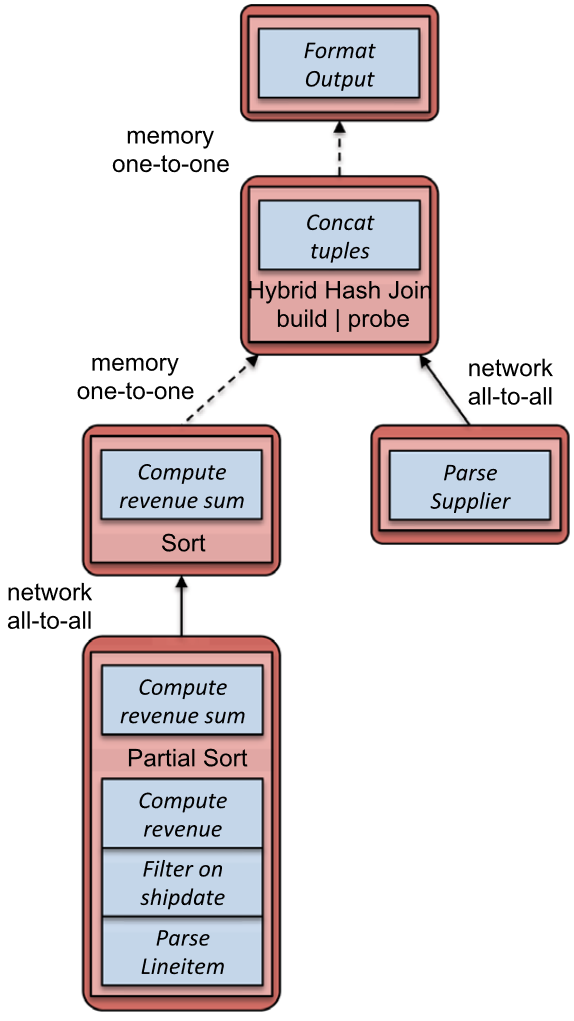
\includegraphics[width=2in]{./img/NepheleDAG.png}
\caption{The Nephele job graph is created after optimization and contains information about how and where to physically execute the query~\cite{Stratosphere2014}.}
\label{fig_stratosphere_nephele_dag}
\end{figure}

The last optimization step results in the Nephele Job Graph (Fig.~\ref{fig_stratosphere_nephele_dag}). Local operations are clustered together to signalize that they form one execution unit. All data forwarding techniques are added to the graph and it is forwarded to Nephele.

\subsection{Nephele}\label{straotsphereNephele}

\begin{figure}[!t]
\centering
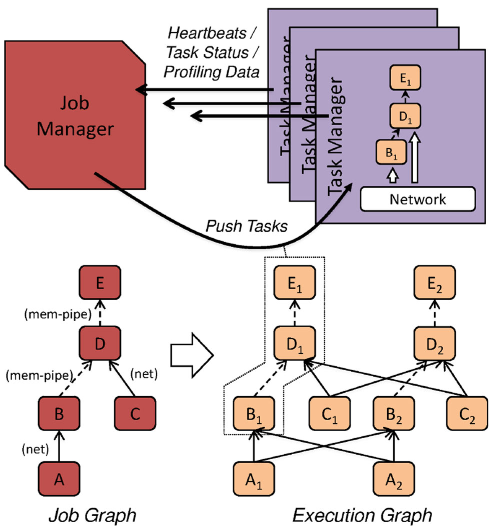
\includegraphics[width=2.5in]{./img/NepheleMasterWorker.png}
\caption{Nephele's job manager assigns tasks to different task managers. One task might be executed on different workers in parallel~\cite{Stratosphere2014}.}
\label{fig_stratosphere_nephele_master_worker}
\end{figure}

Nephele is Stratosphere's distributed execution engine. It takes a Nephele Job Graph as input. The system uses a master/worker pattern to distribute tasks and the necessary communication is provided via messaging. Fig.~\ref{fig_stratosphere_nephele_master_worker} shows that there is one Job Manager that assigns tasks to the different task managers, which represent different nodes in a distributed system. In the beginning, Nephele assigns the jobs containing the data sources to different Task Managers. The following tasks are executed lazily: when a Task Manager has finished its job and asks the Job Manager where to forward their data, the succeeding tasks are started, if they have not already. When sending data via network, Task Managers are able to compress the data to minimize network throughput. This is a tradeoff between computing power to compress and decompress data and network load.

To provide fault tolerance, Nephele works with log-based rollback recovery, similar to other data flow engines, such as Hadoop~\footnote{https://hadoop.apache.org/}, Spark~\footnote{https://spark.apache.org/} and Dryad~\footnote{https://www.microsoft.com/en-us/research/project/dryad/}. The main difference in Stratosphere is that operators are non-blocking, which means that tuples get forwarded as soon as they have been processed at the preceding operator. In a case of failure, some tuples might not have been processed yet, while other might have already been forwarded to following operators. Nephele keeps track of tuples already processed by an operator with a duplication detection system similar to TCP. For the rollback, the optimizer is able to identify possible checkpoints for materialization of intermediate results. Sometimes, however, materializing costs are higher than recomputation costs, leading to the checkpoint being ignored.

Stratosphere is implemented in Java. While this, because of the extensive libraries and far evolved language, is a good fit for programming UDFs, some difficulties arise with regard to core system functionalities of Stratosphere. Java does not support explicit memory control and Java-objects tend to have a large memory overhead. Further, the Garbage Collector needs much memory. Those issues are addressed by careful usage of the Java language. For example, the developers decided to use large byte arrays to reduce object overhead and minimize the Garbage Collectors activity by lazily deserializing fields of the byte arrays into objects.

\subsection{Stratosphere performance}\label{straotspherePerformance}
The developers tested Stratosphere against Apache Hadoop's MapReduce~\footnote{\url{https://hadoop.apache.org/docs/r1.2.1/index.html#MapReduce}}, Apache Hive~\footnote{\url{https://hive.apache.org/}} and Apache Giraph~\footnote{\url{https://giraph.apache.org/}} in different benchmarks, such as TeraSort, Word Count, a relational query, triangle enumeration of a graph, and a connected components algorithm. The results have shown that Stratosphere has comparable or better performance than the competitors. As a reason, the authors have identified execution layer features, such as PACT implementations and the push-based communication between Task Managers.

\subsection{Areas for improvement in Stratosphere}\label{stratosphereImprovement}
In 2014, the authors defined some areas for further research. They wanted to add support for a functional programming language (for PACT). Also, they experimented with porting existing high level declarative languages to Stratosphere. One major research was unifying the Sopremo and PACT layer into a single model, that should support user defined functions as well as operators with known semantics. Another major area was defined as improving fault tolerance by introducing an adaptive algorithm, that picks the intermediate to materialize and is able to take different statistics into account. To the best of our knowledge, many of those goals have been implemented in later Stratosphere versions (support for functional programming language SCALA~\footnote{\url{https://dms.sztaki.hu/sites/dms.sztaki.hu/files/file/2014/stratosphere_meetup.pdf}. Last accessed on 06.07.2019. In this presentation, the author uses SCALA to present the system.}) and afterwards Apache Flink~\cite{Flink2015}.